\section{作成したシステムの概要}
\subsection{光センサによる居眠り検知}
\subsubsection{システムの概要}

光センサによる居眠り検知・防止装置の大まかな仕組みは，図\ref{fig1}に示す通りである．
この装置は，2つの光センサ（Cdsセル）を使用する．これまで覚醒度低下の検出に光センサを用いた例は見当たらず，簡易に実現できるため，この点において本装置は新規性があると考える．
光センサの一つ目は，部屋の明るさを検知するための光センサAである．光センサAは，図\ref{fig1}のように物体の影にならないように配置する．しかし，光センサAの値は，他人が傍を通るだけで容易に変化してしまう．
よって，システムの各条件に用いる環境光（Ambient\_Light）は，光センサAの分散が一定以上小さくなった時の光センサAの平均値とする．
予備実験として，本装置を用いて動作確認をした結果，光センサAの値が安定した時の分散の値は，
0または1であったため，光センサAの分散の条件は1以下とした．二つ目は，頭の動きを検知する光センサBである．
光センサBが設置されたボックスには安全ピンがついており，衣服に装着して使用する．
\begin{figure}[bt]
\begin{center}
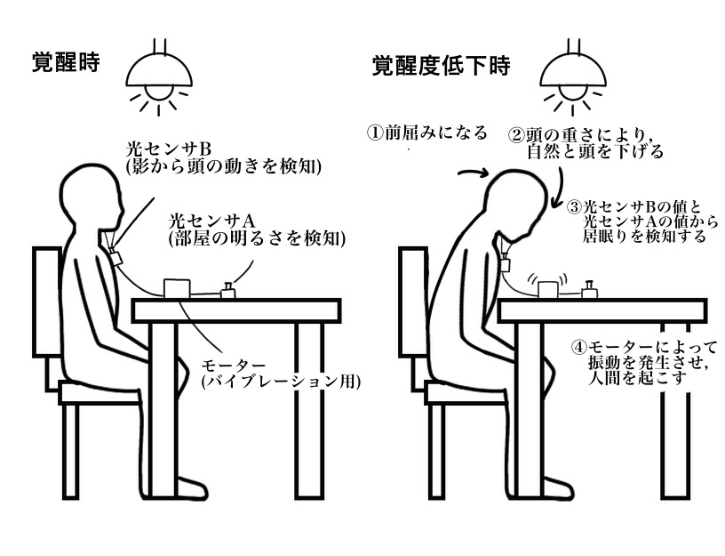
\includegraphics[width=13cm, clip]{fig1.pdf}
\caption{覚醒時と覚醒度低下時のシステムの動作}
\label{fig1}
\end{center}
\end{figure}

まず，覚醒度低下時のシステムの動作を説明する．図\ref{fig1}の右側のように，覚醒度低下時は，人は頭の重さによって下を向いたり前かがみになることが自然である．前かがみになると，光センサBの値が環境光の光センサAの値よりも小さくなる．本システムはこの値の差を用い，2.1.2節で説明する方法によって居眠り状態を検出する．居眠り状態が検出されると，モータを回転させて振動を起こし，使用者の居眠り防止を図る．


次に，誤使用時のシステムの動作を説明する．ここでいう``誤使用時''とは，図\ref{fig2}のように使用者の姿勢が悪い時，光センサAが物影にある時などを指す．いずれも光センサBの値が環境光よりも大きくなるような場合である．この時，光センサによる居眠り検知・防止は正しく行えないため，モータによる振動で使用者に問題を解決するよう警告する．この点において，誤使用を検知できずに乱数値を出力する脈拍センサよりも有効性があると言える．また，正しく装着していても頭を動かすことにより，光センサBが環境光よりも値を大きく取ってしまう場合がある．そのような状況と誤使用を区別するため，条件として5秒間毎の光センサBの分散（頭の動きの大きさ）が1以下であることを加える．
\begin{figure}[bt]
\begin{center}
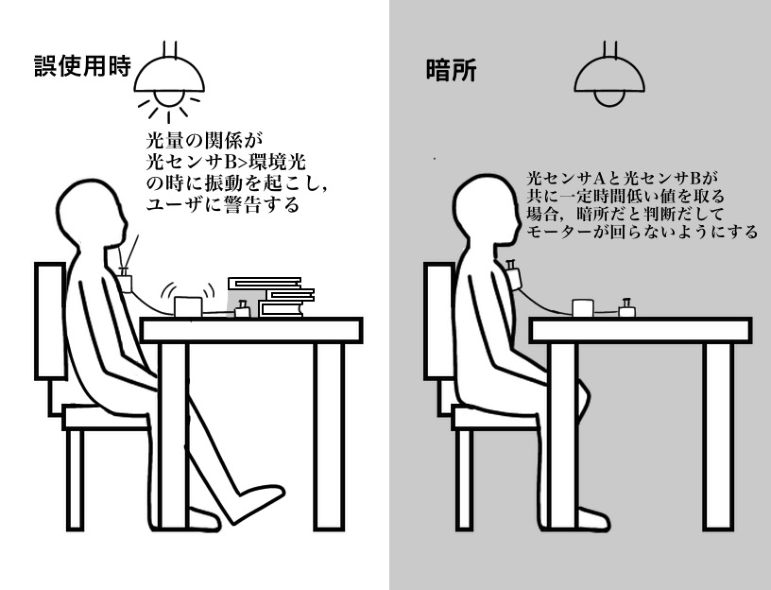
\includegraphics[width=13cm, clip]{fig2.pdf}
\caption{姿勢が悪い時と暗所にいる際のシステムの動作}
\label{fig2}
\end{center}
\end{figure}


最後に暗所にいる際のシステムの動作を説明する．本装置は，昼食後のデスクワークにおける居眠り検知・防止を想定しているため，暗所時は動作しないこととする．具体的には，5秒間の光センサAの平均値と光センサBの平均値がともに閾値（Night\_Mode\_Value）より小さい場合に暗所と判断し，誤ってモータが回らないようにする．実際には，予備実験により暗いと感じた時の光センサの値を調べNight\_Mode\_Valueは15と設定した．

\subsubsection{頭の影と環境光の関係と居眠り判定法}

光センサによる居眠り判定の条件を考案するために，頭の影と環境光の光量の関係を導いた．二つの光センサ（Cdsセル）を用意し，2.1.1節で説明したシステムと同様に机の上に光センサAを，首元に光センサBを設置した．正しい姿勢を維持したまま，部屋の明るさ（環境光）のみを4段階変化させ，二つの光センサの光量を5分おきに5回記録した．それぞれの段階の平均値の結果を表\ref{tab1}に示す．
表\ref{tab1}に示された“環境光の平均値/光センサBの値の平均値“の4つの結果をみると，環境光と光センサBの値は一定の比率があることが読み取れる．“環境光の平均値/光センサBの値の平均値“をさらに平均すると2.96となる．ここから，実験を行った部屋における環境光の光量は，頭の影の光量の3倍であるという関係性があることがわかる．また，部屋の明るさによらず，環境光と頭の影の比率は，変わらないことも読み取れる．
この結果から，光センサによる居眠り検知の判定方法は，光センサBの値が環境光に比べ，何倍であるかに注目すればよいことがわかる．そこで，居眠りの体勢をとった状態における光センサBの値と環境光の値を同様の条件で計測した．その結果を平均したものを表\ref{tab2}に示す．

\begin{table}[bt]
\caption{環境光と頭の影の光量の関係}
\label{tab1}
\begin{tabular}{|r|r|r|}\hline
環境光の平均値&光センサBの値の平均値&環境光の平均値/光センサBの値の平均値\\ \hline
54.2&19.8&2.73\\
42.6&14.4&2.94\\
32.0&10.4&3.07\\
24.2&7.8&3.1\\ \hline
\end{tabular}
\end{table}


表\ref{tab2}に示された“環境光の平均値/光センサBの値の平均値”の4つ結果をさらに平均すると4.017となる．ここから，実験を行った部屋における環境光の光量は，頭の影の光量の4倍であるという関係性があることがわかる．よって，居眠り判定の閾値を環境光の4分の1とした．
また，光センサBの値と環境光の比較のみを居眠りの条件としてしまうと，覚醒時に頭を動かした際に誤って居眠りと判定してしまう場合がある．使用者がうとうとして前かがみになり，頭が動かなくなった時点を居眠りと判定するため，居眠りの判定条件に5秒間ごとの光センサBの値の分散が1以下であることを加えることとする．

\begin{table}[bt]
\caption{環境光と下を向いた頭の影の光量の関係}
\label{tab2}
\begin{tabular}{|r|r|r|}\hline
環境光の平均値&光センサBの値の平均値&環境光の平均値/光センサBの値の平均値\\ \hline
55.6&13.2&4.21\\
43.8&9.4&4.65\\
33.0&8.4&3.928\\
25.0&7.6&3.28\\ \hline
\end{tabular}

\end{table}

\subsection{脈拍センサによる居眠り推定法}
\subsubsection{心拍間隔の定義}

居眠り検知に使われている生理情報の一つとして，心拍変動（HRV: heart rate variability）がある．HRVは，心電図や脈波等から計測した心拍周期の変動を解析するものである．心電図（ECG: Electrocardiogram）の概略図を図\ref{fig3}に示す\cite{[7]}\cite{[9]}．この電気信号は，心臓が収縮する際に生じる電気の分布の変化によって引き起こされる\cite{[10]}．この電気信号には，P，Q，R，S，Tといった名称がつけられており，特に図\ref{fig3}に示す波形のピークはRと呼ばれる．一般にR波は，心拍の間隔を計測する際に利用される．R波同士の時間間隔のことをRRI（R-R Interval）と呼び，これが心拍間隔に相当する．

\begin{figure}[bt]
\begin{center}
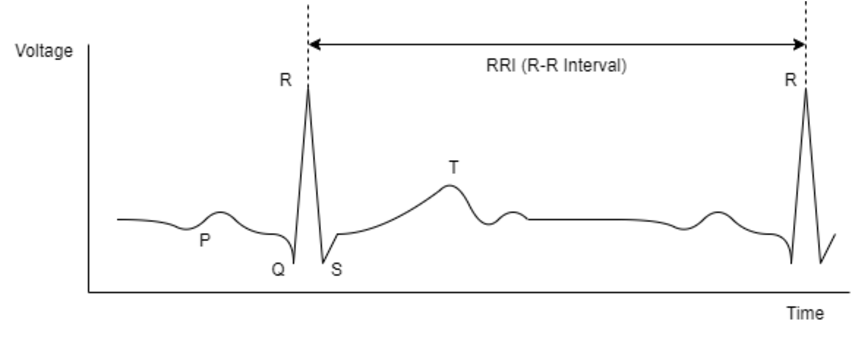
\includegraphics[width=14cm, clip]{fig3.pdf}
\caption{RRI（R-R Interval）}
\label{fig3}
\end{center}
\end{figure}

\subsubsection{LPとは}

HRV解析の時間領域指標の一つにローレンツプロット（LP: Lorenz plot）がある．LPは，ポアンカレプロットとも呼ばれる．これは，RRIの変動を視覚的に捉える幾何学図形解析手法であり，不整脈自動解析，心臓自律神経機能解析，睡眠状態の解析等に用いられている\cite{[9]}．具体的には，図\ref{fig4}に示すように，$n$番目のRRIをX座標，$n+1$番目のRRIをY座標とし，心拍に対してx-y平面上に順にプロットしたものである．通常，LPは直線$RRI_{n+1}=RRI_n$を長軸とした楕円状に分布することが知られている.また，一般に安静時はプロットの重心が右上に推移し，緊張時は左下方向に推移しながら各点の散らばりが大きくなる．さらに緊張が高まると，プロットの重心は左下に推移しながら各点の散らばりが小さくなることが知られている．

\subsubsection{F-stressの実装}

2.2.2で説明したLPの性質を考慮し，松本佳昭らは評価関数F-stressを提案した\cite{[9]}．
まず，（1）式に示すように，プロットの原点から重心までの距離を$g_p$とする．さらに，（2）式で示すように，重心と各点のばらつきを表す指標として，各点から重心までの平均距離を$\delta$とする．これらの特徴量を（3）式のように積をとったものをF-stressとする．
\begin{equation}
g_p = \sqrt{X_G^2 + Y_G^2}
\end{equation}
ただし，
\begin{equation}
X_G = \frac{1}{n}\sum^{n-1}_{i=0}X_i,   Y_G = \frac{1}{n}\sum^{n-1}_{i=0}X_i
\end{equation}
\begin{equation}
\delta = \frac{1}{n}\sum^{n-1}_{i=0}\sqrt{(X_G-X_i)^2 + (Y_G-Y_i)^2}
\end{equation}
\begin{equation}
F_\mathrm{stress} = g_p\cdot \delta
\end{equation}

ここで，論文\cite{[9]}では$g_p$と$\delta$は，それぞれ0～1に正規化したものを用いている．しかし，本実験では，ProcessingでF-stressの変動をより見やすくするために0～1正規化を行わないこととする．また，Processingでの表示の都合上，Arduino側でF-stressを5で割った値をProcessingに送信するようにしている．これは，表示するためだけに値の大きさを変更しているため，本来の値の変動自体に影響を与えない．論文\cite{[9]}によると，この評価値がゼロに近くなるほど，ストレスが高まっていることになる．Arduino側でのF-stressを算出する関数を図\ref{sk1}に示す．
\begin{figure}[tb]
\begin{center}
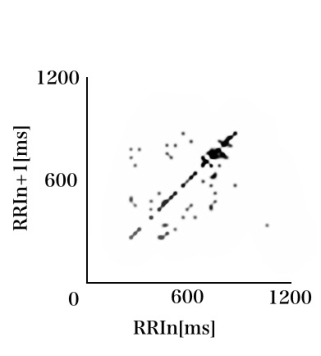
\includegraphics[width=5cm, clip]{fig4.pdf}
\caption{ローレンツプロット（LP）}
\label{fig4}
\end{center}
\end{figure}

\begin{figure}[tb]
\begin{lstlisting}
1:	int Check_F_stress(){//ストレス値を計算
2:	 float delta=0;
3:	 float G_p,G_x,G_y;//G_pは重心
4:	 int F_stress;
5:	 int sum_x =0,sum_y=0;
6:	 int i;
7:	
8:	 for(i = check_range - 2; i >= 0 ;i--){
9:	  sum_x += Data_IBI[i];
10:	  sum_y += Data_IBI[i+1];
11:	 }
12:	 G_x = sum_x/(check_range - 1);
13:	 G_y = sum_y/(check_range - 1);
14:	 G_p = G_x*G_x + G_y*G_y;
15:	 G_p = sqrt(G_p);
16:	 for(i=check_range - 2; i >= 0 ;i--){
17:	   delta = delta + (G_x - Data_IBI[i])*(G_x - Data_IBI[i]) 
               + (G_y - Data_IBI[i+1])*(G_y - Data_IBI[i+1]);
18:	 }
19:	 delta = sqrt(delta);
20:	 delta = delta /(check_range - 1 );
21:	 F_stress = delta*G_p/5;
22:	 return F_stress;23:	}
\end{lstlisting}
\caption{スケッチ1: F-stressの関数}
\label{sk1}
\end{figure}

\subsection{システムの実装}
\subsubsection{フローチャートと関数の機能}

Arduino側の主要な処理で用いる関数を次のように定義する．
\begin{description}
\item[loop()関数]
センサから値を読み取り，その値を送信できる形に変換する．その後，シリアル通信を用いてProcessingへ送信する．Check\_F\_stress()やCheck\_Data()などの各関数を呼び出す．尚，この関数は繰り返し実行される．
フローチャートを図\ref{fig6}に示す．
\item[Check\_F\_stress()関数]
RRIから計算できるストレス値を算出する．フローチャートを図\ref{fig7}に示す．
\item[Check\_DataA\_Variation()関数]
5秒間の光センサAの平均値と5秒間ごとの分散を求め，分散が1以下になった時の平均値を環境光として設定する．フローチャートを図\ref{fig8}に示す．
\item[Check\_DataB()関数]
5秒間の光センサBの平均値と5秒間ごとの分散を求め，暗所モード判定，居眠り判定，誤使用判定等を行う．フローチャートを図\ref{fig9}に示す．
\end{description}

\begin{figure}[p]
\begin{center}
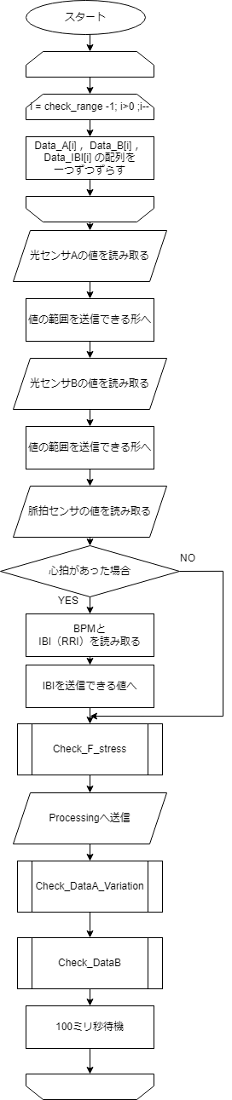
\includegraphics[width=4cm, clip]{fig5.png}
\caption{loop()関数のフローチャート}
\label{fig6}
\end{center}
\end{figure}

\begin{figure}[p]
\begin{center}
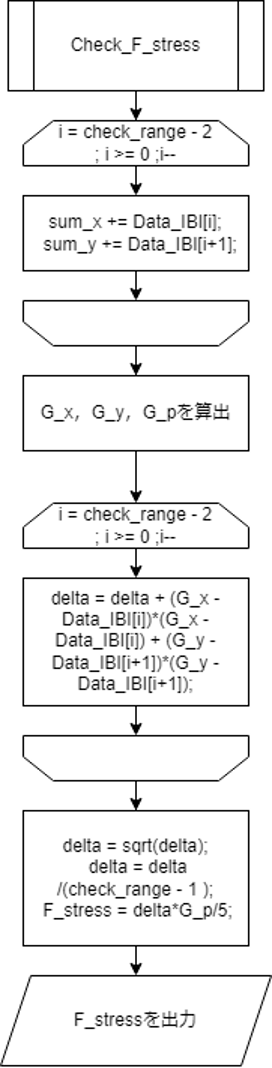
\includegraphics[width=4cm, clip]{fig6.png}
\caption{Check\_F\_stress()関数のフローチャート}
\label{fig7}
\end{center}
\end{figure}

\begin{figure}[p]
\begin{center}
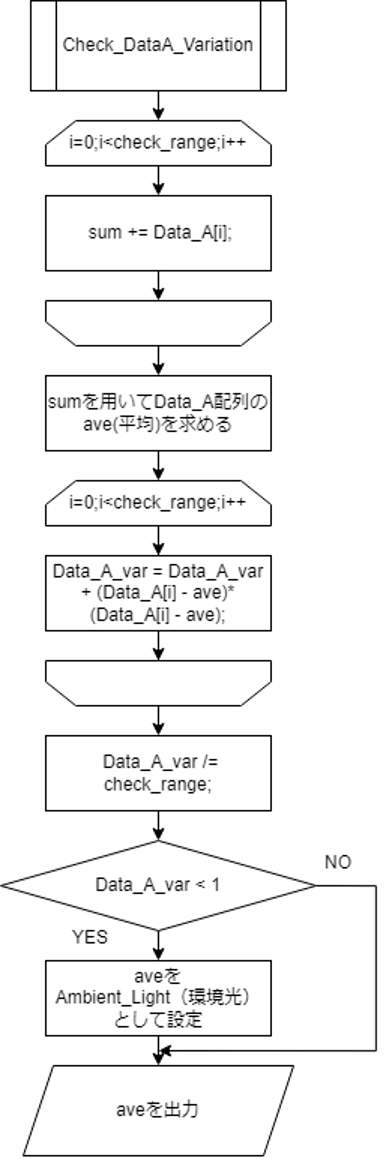
\includegraphics[width=7cm, clip]{fig7.png}
\caption{Check\_DataA\_Variation()関数のフローチャート}
\label{fig8}
\end{center}
\end{figure}

\begin{figure}[p]
\begin{center}
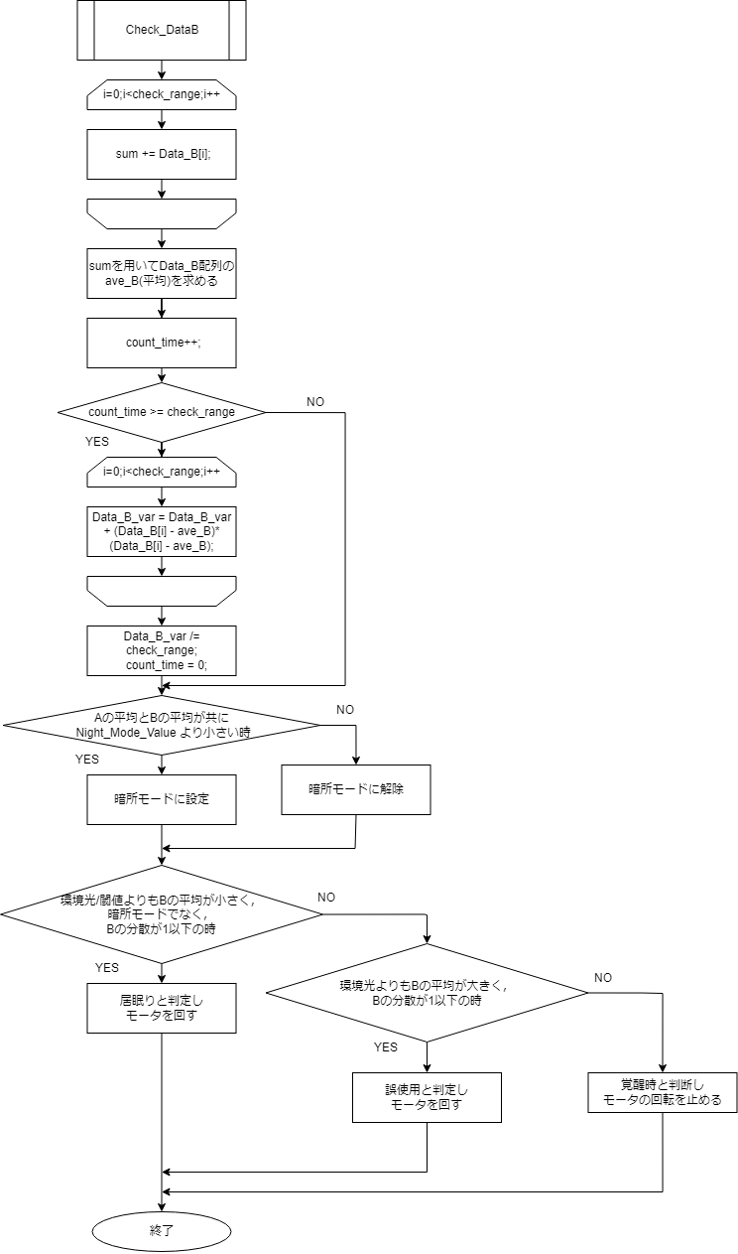
\includegraphics[width=11cm, clip]{fig8.png}
\caption{Check\_DataB()関数のフローチャート}
\label{fig9}
\end{center}
\end{figure}


\subsubsection{Processing側での表示の工夫}

多くのデータをシリアル通信していると値にノイズが入ることがある．例えば，光センサBの値の分散（Data\_B\_var）をProcessing側で表示すると，“$-1$”という値が画面上でチラつくことがある．そこで，図\ref{sk2}に示すように工夫を施した．Data\_B\_varが$-1$であるならば，過去のBの値の分散(Data\_B\_var\_pr)を表示し，Data\_B\_varが$-1$でないならば，Data\_B\_var\_prを更新して現在のBの値の分散（Data\_B\_var）を表示する．こうすることにより，$-1$のチラつきを抑えることができた．

\begin{figure}[tb]
\begin{lstlisting}
1:	fill(255,0,0);
2:	textSize(16);
3:	if(Data_B_var != -1){
4:	Data_B_var_pr = Data_B_var;
5:	 text("Data_B_var:" + str(Data_B_var),140,20);
6:	}else{
7:	text("Data_B_var:" + str(Data_B_var_pr),140,20);8:	}
\end{lstlisting}
\caption{ノイズ除去}
\label{sk2}
\end{figure}

\subsubsection{回路図と用いた機器}

用いた機器を表\ref{tab4}に示す．また，回路図を図\ref{kairo}に示す．
\begin{table}[bt]
\centering
\caption{主な関数と機能}
\label{tab4}
\begin{tabular}{|l|l|}\hline
機器&個数\\ \hline
Arduino Uno & 1\\
ブレッドボード&4\\
DCモータ（FA-130RAL）&1\\
モータドライバ（TA7291P）&1\\
光センサ（Cdsセル）&2\\
脈拍センサ（SFE-SEN-11574）&1\\
抵抗（1k$\Omega$）&2\\
抵抗（10k$\Omega$）&1\\ \hline
\end{tabular}
\end{table}

\begin{figure}[bt]
\begin{center}
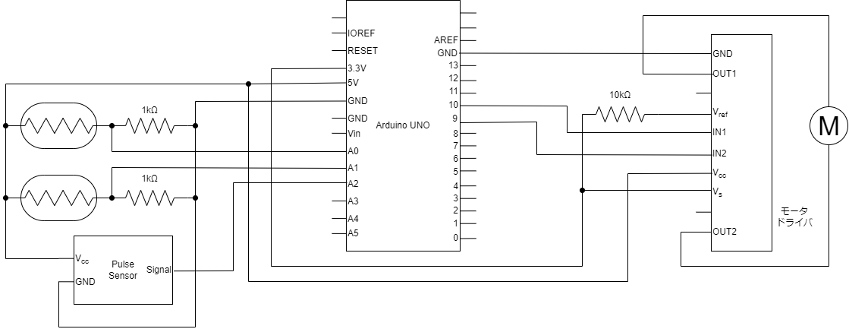
\includegraphics[width=13cm, clip]{fig9.png}
\caption{システムの回路図}
\label{kairo}
\end{center}
\end{figure}

